\documentclass{article}
\documentclass{memoir}
\usepackage{graphicx} % Required for inserting images
\usepackage{titling}% the wheel somebody else kindly made for us earlier
%\usepackage{titlepic}
\usepackage{fancyhdr}
\usepackage{tikz}
\usetikzlibrary{chains,arrows,shapes,positioning}
\usepackage{hyperref}
\usepackage{geometry}
\geometry{margin=2cm}

\pretitle{% add some rules
  \begin{center}
    \Huge\bfseries}
%, make the fonts bigger, make the title (only) bold

\posttitle{%
  \end{center}%
  \noindent\vrule height 2.5pt width \textwidth
  \vskip .75em plus .25em minus .25em% increase the vertical spacing a bit, make this particular glue stretchier
}



\title{User guide Digi-Sm}
\author{Benjamin Richter}
\date{April 2023}



\begin{document}

\maketitle


\vfill

\begin{center}
    \includegraphics[width=9cm]{logo1.png}
\end{center}



\newpage





\tableofcontents
\clearpage


\section{Introduction}

The Digi-SM user guide is a comprehensive resource that helps programmers and project managers learn and apply the Agile methodology to their projects. It provides step-by-step instructions for using the Digi-SM website, including how to register, create projects/user stories as well as creating and managing sprints. The guide also includes information on additional features such as team management, adding friends, profiles, and notifications. There is a glossary of terms at the end of the guide as well as a list of frequently asked questions to help users troubleshoot common issues.


\section{What is Digi-Sm}

Digi-SM, short for Digital Scrum Master, is a powerful and intuitive website designed to help you and your team develop projects and implement the Agile methodology with ease. With Digi-SM, you can effectively manage all aspects of your project development process, from creating user stories to organizing sprints, tracking progress and visualising this data through graphs and diagrams.\\

One of the main benefits of Digi-Sm is its simple and user friendly interface. You can easily create an account and get straight to work from any device connected to the internet. This allows your team to spend less time on planning and thus more time on getting your project on track! \\

Digi-SM's project management features are designed to help you and your team stay on track and organized throughout the development process. You can create and input all of your user stories at once, making it easy to see at a glance what needs to be done and when.\\

Whether you're just starting out or looking to streamline your existing processes, Digi-SM can help you and your team achieve your project development goals.\\



\newpage


\section{Quickstart}\label{quickstart}



\subsection{Workflow}

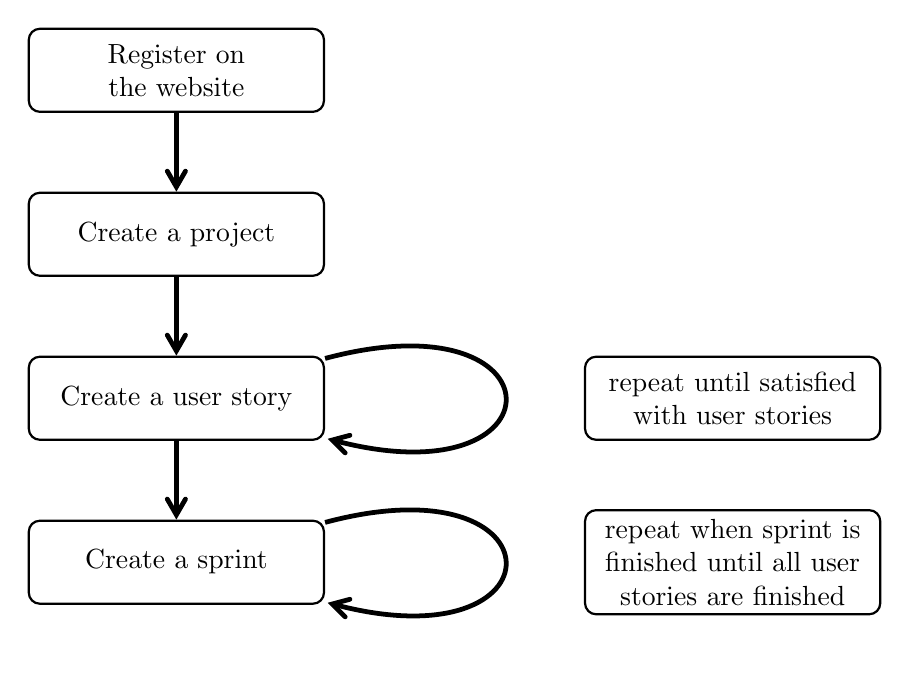
\begin{tikzpicture}
\tikzset{every node/.style={on chain,draw,thick,rounded corners,
minimum height=3em, text width=10em, align=center}}
\begin{scope}[start chain=going below]
\node (Register on the website) {Register on the website};
\node (Create a project) {Create a project};
\node (Create user story) {Create a user story};
\node (Create a sprint) {Create a sprint};
\end{scope}
%\node[right=of Create user story] (open-score) {Open previously saved score file (\texttt{.xml})};

\path[draw,line width=0.4ex, ->,>= angle 60]
(Register on the website) edge (Create a project) 
(Create a project) edge (Create user story)
(Create user story) edge [loop right] node [right= of Create user story] {repeat until satisfied with user stories} (Create user story)
(Create user story) edge  (Create a sprint)
(Create a sprint) edge [loop right] node [right= of Create a sprint] {repeat when sprint is finished until all user stories are finished} (Create a sprint);
\end{tikzpicture}



\subsection{Registering}

To get started with Digi-SM, you'll first need to create an account. \\

\begin{enumerate}
    \item Visit the Digi-SM website and click on the "Register" button.\\
    \includegraphics[width=10cm]{registering.png}
    \newpage
    \item Fill in your details and click on "Register" to complete the process.\\
    \includegraphics[width=10cm]{registerInfo.png}
    \item Once you're registered, you'll be able to log in and start using the platform right away.
\end{enumerate}



\subsection{Create a project}

After you've registered or logged-in to Digi-SM, creating a new project is easy as you'll be automatically redirected to the page seen below, which is the project management page.\\

\begin{enumerate}
    \item Click on the "New Project" button in the navigation bar.\\\\
    \includegraphics[width=10cm]{newProjectNav.png}
    \item Enter a name and a description for your project.\\\\
    \includegraphics[width=10cm]{createProject.png}
    \item Once you've filled in all the details, click on "Submit" to get started. 
\end{enumerate}

\newpage

\subsection{Create a user story}

User stories are an essential part of the Agile methodology, and Digi-SM makes it easy to create and manage them.\\

\begin{enumerate}
    \item To create a new user story, simply click on the "New User Story" button in the navigation bar.\\\\
    \includegraphics[width=10cm]{userStoryNav.png}
    \item Enter a title, description, and poker score based on the perceived difficulty.\\\\
    \includegraphics[width=10cm]{userStory.png}
    \item  Once you've filled in all the details, click on "Submit" to add it to your project.
\end{enumerate} 



\subsection{Create a sprint}

Sprints are a key part of the Agile methodology, and Digi-SM makes it easy to create and manage them. 

\begin{enumerate}
    \item To create a new sprint, simply click on the "Create New Sprint" button in the navigation bar.\\\\
    \includegraphics[width=10cm]{sprintNav.png}
    \item Then simply assign user stories to it by clicking the rows. The selected rows will then be highlighted to indicate that they have indeed been selected.\\\\
    \includegraphics[width=10cm]{createSprint.png}
    \item  Once you’ve selected the user stories simply click on create sprint.
\end{enumerate}


We hope this quick start guide has helped you get started with Digi-SM. If you have any more questions you can keep reading or head to the FAQ section at the bottom. Happy developing!

\newpage

\section{Further features}

\subsection{Manage your team}

Digi-SM makes it easy to manage your team. To add team members to a project:

\begin{enumerate}
    \item Select the "Team" button in the navigation bar.\\\\
    \includegraphics[width=10cm]{teamNav.png}
    \item From here, you can view a list of existing team members and add new ones by entering their username in the text field pictured below. \\\\
    \includegraphics[width=10cm]{team.png}
    \item Once they’ve accepted the request you can both work on the project simultaneously!
\end{enumerate}

\newpage

\subsection{Friend list}

Digi-SM also makes it easy to connect with other users and add them as friends. 

\begin{enumerate}
    \item To view your friend list, click on the "Friends" tab on the dashboard.\\\\
    \includegraphics[width=10cm]{friendsNav.png}
    \item From here, you can view a list of your current friends and add new ones by searching for their username.\\\\
    \includegraphics[width=10cm]{friends.png}
    \item Once you've added a friend, you can view them in your list and add them to your projects.
\end{enumerate}

\newpage

\subsection{Profile page}

Your profile page is where you can manage your personal information and customize your Digi-SM experience. 

\begin{enumerate}
    \item To access your profile, click on the profile button which you can find on the right-hand side of your navigation bar at the top of your screen.\\\\
    \includegraphics[width=10cm]{profileNav.png}
    \item From here, you can edit your personal information.\\\\
    \includegraphics[width=10cm]{personalInfo.png}
    \item You can also change your password here.\\\\
    \includegraphics[width=10cm]{password.png}
\end{enumerate}  

\newpage

\subsection{Notifications}

Digi-SM notifies you of all the requests you've received, whether its project or a friend request, through its\\ notification system. To view your notifications:

\begin{enumerate}
    \item Click on the  \includegraphics[width=0.3cm]{bell-solid.png}  icon in the top right corner of the screen.\\\
    \includegraphics[width=10cm]{notificationNav.png}
    \item From here, you can view requests from other users and accept or reject them with a single click.\\\\
    \includegraphics[width=10cm]{notification.png}
\end{enumerate}  



\subsection{Timeline}

The timeline serves as an interactive graphic to visualise the sprints of the project. The currently selected sprint is highlighted and the other ones can be selected by clicking directly on them. \\\\
\includegraphics[width=10cm]{timeline.png}

If you have more than 5 sprints a scroll feature will automatically be enabled with which you can load 5 sprints at a time and go forward and backward in time. As you can see the "future sprints" button has been transformed into a "later sprints" button which you can select to load the next set of sprints.\\\\
\includegraphics[width=10cm]{timelineMore.png}\\\\\\

We hope this guide has helped you get started with Digi-SM's team, friend, profile, and notification features. If you have any further questions or need assistance, don't hesitate to contact our \hyperref[sec:ContactInfo]{support team}. Happy developing!

\newpage

\section{FAQ}

\subsection{What is Digi-Sm?}

\subsubsection{How do I get started with Digi-SM?}

The heart of the website is the management of projects, so the best way to get going is to create your first project and to mess around with the website a bit.
This being said you can check the quickstart guide on page \pageref{quickstart}.


\subsubsection{How can this website help me?}

This website is designed to organize and plan your projects methodically. On top of this the website is filled with tips and tricks to help you develop some good development habits. If you look around the website you can find some \includegraphics[width=0.3cm]{questionMark.png} icons scattered around the website next to foreign or terms relating to the agile development methodology. Simply click on them and you'll be able to read a brief tutorial on the subject.

\subsection{Features of the website}

\subsubsection{Can I export the analytics generated by the website?}

Not yet- Digi-SM offer a variety of metrics to track the advancement of your project. These have been simplified thanks to the two main visuals available from the front page and are easily accessible once you've loaded your project, but cannot be exported yet. 

\subsubsection{Can I mark a sprint as finished?}

Yes and no- your sprints are done if all the user stories within them are marked as Done. You can see this by loading the pie chart which allows you to quickly visualise what user stories are left to accomplish, are still being worked on or are finished.
So there is a way to visualise it yes but no there is no directly accessible metric.


\subsubsection{Can I change my password?}

Yes- Once on the homepage press the "Profile" button in the top right corner of your screen. Once on the profile page you’ll see your information is loaded. The two fields at the bottom is where you can enter your new password and its confirmation in order to change it.

\subsection{Learning to be an agile developer}

\subsubsection{Where can I get more information about the agile methodology?}

The agile methodology is very flexible and usually everyone has their own variant of the technique. This being said you can learn the template of the agile methodology through the tutorial spread throughout the website. Just lookout for the little blue question marks.
And if you need any more information you can head to https://www.atlassian.com/agile which is a wonderful source of information.

\subsection{Contact information}
\label{sec:ContactInfo}

\subsubsection{How can I contact support if I have any questions or issues with Digi-SM?
}

This is an open-source project realised for a bachelor project. This means that there is no team which will be able to answer quickly but you can reach me at benjamin.richter@student.unamur.be and I'll come back to you as quickly as I can.

\newpage

\section{Glossary of terms}

\begin{enumerate}
\item Agile methodology: An iterative approach to project management that emphasizes collaboration, flexibility, and customer satisfaction.
\item Backlog: A list of prioritized tasks or user stories that need to be completed in a project.
\item Burndown chart: A visual representation of the amount of work remaining in a sprint or project, typically plotted against a timeline.
\item Scrum: A framework for Agile project management that emphasizes teamwork, accountability, and regular progress reviews.
\item Sprint: A time-boxed period (usually 1-4 weeks) during which a team works to complete a set of tasks or user stories.
\item User story: A short, simple description of a feature or requirement from the perspective of an end user.
\end{enumerate}

\end{document}
